%%*************************************************************************
%% The Berkeley Out-of-Order Machine
%% Christopher Celio
%% 2015 Dec 17
%% 
%% Design document
%%*************************************************************************


\documentclass[11pt, notitlepage]{report}


\usepackage{graphicx}
\usepackage{url}
\usepackage{fullpage}
\usepackage{listings} % used for putting code
\usepackage{color}
\usepackage[multiple]{footmisc}
%\usepackage{wrapfig} % allow text to wrap around a figure

\usepackage{hyperref} 
\hypersetup{
    colorlinks=true,
    linkcolor=black,
    urlcolor=red,
    citecolor=black,
    filecolor=black,
    linktoc=all
}

\let\tt\texttt

\lstset{ %
language=C++,                % choose the language of the code
%basicstyle=\small\ttfamily,      % the size of the fonts that are used for the code
basicstyle=\scriptsize\ttfamily,basewidth=0.50em,      % the size of the fonts that are used for the code
numbers=left,                   % where to put the line-numbers
numberstyle=\scriptsize,      % the size of the fonts that are used for the line-numbers
stepnumber=1,                   % the step between two line-numbers. If it is 1 each line will be numbered
numbersep=5pt,                  % how far the line-numbers are from the code
backgroundcolor=\color{white},  % choose the background color. You must add \usepackage{color}
showspaces=false,               % show spaces adding particular underscores
showstringspaces=false,         % underline spaces within strings
showtabs=false,                 % show tabs within strings adding particular underscores
frame=single,                   % adds a frame around the code
tabsize=3,              % sets default tabsize to 3 spaces
captionpos=b,                   % sets the caption-position to bottom
breaklines=true,        % sets automatic line breaking
breakatwhitespace=false,    % sets if automatic breaks should only happen at whitespace
linewidth=1.0\textwidth,
boxpos=b,
%escapeinside={\%
%}
%{
%)}          % if you want to add a comment within your code
}
\renewcommand{\lstlistingname}{Code} % change caption title from 'listings' to what I want



\newcommand{\smalltodo}[1]{\marginpar{\footnotesize #1}}

\newcommand{\TODO}[1]{{\color{red} {\textbf [ TODO: #1 ]}}}
\newcommand{\fixme}[1]{{\color{red} {\textbf [ FIXME: #1 ]}}}
\newcommand{\ooo}{out-of-order}
\newcommand{\boom}{{\em BOOM}}
\newcommand{\BOOM}{{\em BOOM}}
\newcommand{\Chisel}{{\em Chisel}}
\newcommand{\Rocket}{{\em Rocket}}
\newcommand{\rocket}{{\em Rocket}}
\newcommand{\rocketchip}{{\em Rocket-chip}}
\newcommand{\fdiv}{{\tt {fdiv}}}
\newcommand{\ghistory}{{\em {ghistory}}}
\newcommand{\jal}{{\tt {JAL}}}
\newcommand{\jalr}{{\tt {JALR}}}


% allow us to add comentary
\newenvironment{commentary}
{ \vspace{-0.2in}
  \begin{quotation}
  \noindent
  \small \em
  \rule{\linewidth}{1pt}\\
}
{
  \end{quotation}
  \vspace{-0.2in}
}



\let\oldthebibliography=\thebibliography
\let\endoldthebibliography=\endthebibliography
\renewenvironment{thebibliography}[1]{%
  \begin{oldthebibliography}{#1}%
    \setlength{\parskip}{0ex}%
    \setlength{\itemsep}{0ex}%
  }%
  {%
    \end{oldthebibliography}%
  }

%%*************************************************************************
\begin{document}


\title{The Berkeley Out-of-Order Machine (BOOM) Design Specification}
\author{Christopher Celio, David Patterson, and Krste Asanovi\'{c}\\
%School of Electrical and Computer Engineering\\
University of California, Berkeley, California 94720--1770\\
{\tt celio@eecs.berkeley.edu}}

\maketitle

%%*************************************************************************

\

\

{\centerline {\color{red}This draft is a work-in-progress.}}


\vfill

\hrule
\

\noindent The information in this publication is subject to change without notice. 

\noindent This document is available at: \url{https://ccelio.github.io/riscv-boom-doc}.

\

\noindent Copyright \copyright\ 2016 Christopher Celio

\

\noindent This work is licensed under the Creative Commons Attribution 4.0 International License (CC BY 4.0). To view a copy of this license, visit \url{http://creativecommons.org/licenses/by/4.0/}.


\thispagestyle{empty} % suppress page number 

%%*************************************************************************

\tableofcontents


\chapter{Introduction \& Overview}
\label{sec:introduction}

The goal of this document is to describe the design and implementation of the Berkeley Out--of--Order Machine (BOOM). 


 BOOM is heavily inspired by the MIPS R10k and the Alpha 21264 out--of--order processors\cite{alpha21264, mipsr10k}.  Like the R10k and the 21264, BOOM is a unified physical register file design (also known as ``explicit register renaming"). 
 
 The source code to BOOM can be found at (\url{https://ucb-bar.github.io/riscv-boom}).
 

\section{The BOOM Pipeline}


\begin{figure}[ht]
	\centering
	\centerline{\includegraphics[scale =.9] {figures/boom_stages}}
	\caption{ \small The Berkeley Out of Order Machine Processor.}
	\label{fig:boom_stages}
\end{figure}

\vfill
\begin{commentary}
Commentary on design decisions and justifications can be found in paragraphs like this one.
\end{commentary}

Conceptually, BOOM is broken up into 10 stages: {\em Fetch, Decode, Register Rename, Dispatch, Issue, Register Read, Execute, Memory, Writeback,} and {\em Commit}.  However, many of those stages are combined in the current implementation, yielding {\em six} stages: {\em Fetch, Decode/Rename/Dispatch, Issue/RegisterRead, Execute, Memory,} and {\em Writeback} ({\em Commit} occurs asynchronously, so I'm not counting that as part of the ``pipeline").   

\begin{quote}
\begin{description}
\item[Fetch]  Instructions are {\em fetched} from the Instruction Memory and pushed into a FIFO queue, known as the {\em fetch buffer}.\footnote{While the fetch buffer is N-entries deep, it can instantly read out the first instruction on the front of the FIFO.  Put another way, instructions don't need to spend N cycles moving their way through the {\em fetch buffer} if there are no instructions in front of them.}
\item[Decode]
{\em Decode} pulls instructions out of the {\em fetch buffer} and generates the appropriate ``micro-op" to place into the pipeline.\footnote{Because RISC-V is a RISC ISA, currently all instructions generate only a single micro-op. More details on how store micro-ops are handled can be found in Chapter \ref{chapter:memory}.} 

\item[Rename]
 The ISA, or ``logical", register specifiers are then {\em renamed} into ``physical" register specifiers.
  
\item[Dispatch] The micro-op is then {\em dispatched}, or written, into the {\em Issue Window}.  
 
\item[Issue]   Micro-ops sitting in the {\em Issue Window} wait until all of their operands are ready, and are then {\em issued}.\footnote{More precisely, uops that are ready assert their request, and the issue scheduler chooses which uops to issue that cycle.}  This is the beginning of the out--of--order piece of the pipeline.
\item[RF Read]  Issued micro-ops first {\em read} their operands from the unified physical register file (or from the bypass network)... 
\item[Execute] ... and then enter the {\em Execute} stage where the functional units reside.  Issued memory operations perform their address calculations in the {\em Execute} stage, and then store the calculated addresses in the Load/Store Unit which resides in the {\em Memory} stage.  
 
\item[Memory]  The Load/Store Unit consists of three queues: a Load Address Queue (LAQ), a Store Address Queue (SAQ), and a Store Data Queue (SDQ).  Loads are fired to memory when their address is present in the LAQ. Stores are fired to memory at {\em Commit} time (and naturally, stores cannot be {\em committed} until both their address and data have been placed in the SAQ and SDQ).
 
\item[Writeback]  ALU operations and load operations are {\em written} back to the physical register file.

\item[Commit] The Reorder Buffer, or ROB, tracks the status of each instruction in the pipeline.  When the head of the ROB is not-busy, the ROB {\em commits} the instruction.  For stores, the ROB signals to the store at the head of the Store Queue that it can now write its data to memory.
\end{description}
\end{quote}


  
BOOM supports full branch speculation and branch prediction.  Each instruction, no matter where it is in the pipeline,  is accompanied by a branch tag that marks which branches the instruction is ``speculated under". A mispredicted branch requires killing all instructions that depended on that branch.  When a branch instructions passes through {\em Rename}, copies of the {\em Register Rename Table} and the {\em Free List} are made.  On a mispredict, the saved processor state is restored.

Although Figure \ref{fig:boom_stages} shows a simplified pipeline, BOOM implements the RV64G and privileged ISAs, which includes single- and double-precision floating point, atomic memory support, and page-based virtual memory. 



\section{The RISC-V ISA}

BOOM implements the RV64G variant of the RISC-V ISA. This includes the MAFD
extensions and the privileged specification (multiply/divide, AMOs,
load-reserve/store-conditional, single- and double-precision IEEE
754-2008 floating point). More information about the RISC-V
ISA can be found at (\url{http://riscv.org}).

RISC-V provides the following features which make it easy to target with high-performance designs:

\begin{quote}
\begin{description}
\item [Relaxed memory model] This greatly simplifies the Load/Store Unit, which does not need to have loads snoop other loads nor does coherence traffic need to snoop the LSU, as required by sequential consistency.
\item [accrued floating point exception flags] The fp status register does not need to be renamed, nor can FP instructions throw exceptions themselves. 
\item [no integer side-effects] All integer ALU operations exhibit no side-effects, save the writing of the destination register. This prevents the need to rename additional condition state.
\item [no \bf{cmov} or predication] Although predication can lower the branch predictor complexity of small designs, it greatly complicates OoO pipelines, including the addition of a third read port for integer operations.
\item [no implicit register specifiers] Even JAL requires specifying an explicit \tt{rd}. This simplifies rename logic, which prevents either the need to know the instruction first before accessing the rename tables, or it prevents adding more ports to remove the instruction decode off the critical path.
\item [\tt{rs1}, \tt{rs2}, \tt{rs3}, \tt{rd} are always in the same place] This allows decode and rename to proceed in parallel. 

\end{description}
\end{quote}

BOOM (currently) does not implement the ``C" compressed extension nor the ``V" vector extension.

\section{The \Chisel\ Hardware Construction Language}

BOOM is implemented in the \Chisel\ hardware construction language.  More information about \Chisel\ can be found at (\url{http://chisel.eecs.berkeley.edu}). 

\newpage

\section{Quick-start}


To build a BOOM C++ emulator and run BOOM through a couple of simple tests:
\\

%\texttt{\$} \verb=export ROCKETCHIP_ADDONS==\verb="boom"=

\texttt{\$} \verb=git clone https://github.com/ucb-bar/rocket-chip.git=

\texttt{\$} \verb=cd rocket-chip=

\texttt{\$} \verb=git checkout boom=

\texttt{\$} \verb=git submodule update --init=

\texttt{\$} \verb=cd emulator; make run CONFIG==\verb=BOOMConfig=

\

{\bf Note:} this assumes you have already installed the riscv-tools toolchain.  If not, visit (\url{https://github.com/riscv/riscv-tools}).

\section{The BOOM Repository}

The BOOM repository holds the source code to the BOOM core; it is not a full processor and thus is \textbf{NOT A SELF-RUNNING} repository.  To instantiate a BOOM core, the Rocket chip generator found in the rocket-chip git repository must be used (\url{https://github.com/ucb-bar/rocket-chip}), which provides the caches, uncore, and other needed infrastructure to support a full processor.

The BOOM source code can be found in \verb=boom/src/main/scala=.  

The code structure is shown below:

\begin{quote}
\begin{itemize}
\item \verb=boom/src/main/scala=/\begin{itemize}
  \item bpd\_pipeline.scala {\footnotesize \color{red} branch prediction stage.}
  \item brpredictor.scala {\footnotesize \color{red} abstract branch predictor.}
  \item configs.scala {\footnotesize \color{red} BOOM configurations. }
  \item consts.scala {\footnotesize \color{red} constant definitions. }
  \item core.scala {\footnotesize \color{red} the top-level of the processor core.}
  \item dcacheshim.scala {\footnotesize \color{red} the shim between the the core and the dcache.}
  \item decode.scala {\footnotesize \color{red} decode stage.}
  \item execute.scala {\footnotesize \color{red} high-level execution units (made up of FUs).}
  \item fpu.scala {\footnotesize \color{red} floating point unit.}
  \item functional\_unit.scala {\footnotesize \color{red} low-level functional units.}
  \item gshare.scala {\footnotesize \color{red} gshare branch predictor.}
  \item imul.scala {\footnotesize \color{red} integer multiplier.}
  \item issue\_ageordered.scala {\footnotesize \color{red} age-ordered (collasping-queue) issue window implementation.}
  \item issue.scala {\footnotesize \color{red} abstract issue window.}
  \item issue\_slot.scala {\footnotesize \color{red} An issue window slot.}
  \item issue\_unordered.scala {\footnotesize \color{red} un-ordered issue window implementation.}
  \item lsu.scala {\footnotesize \color{red} load/store unit.}
  \item package.scala {\footnotesize \color{red} }
  \item parameters.scala {\footnotesize \color{red} knobs/parameters.}
  \item prefetcher.scala {\footnotesize \color{red} data prefetcher.}
  \item regfile.scala {\footnotesize \color{red} register file.}
  \item registerread.scala {\footnotesize \color{red} registerRead stage and bypassing.}
  \item rename.scala {\footnotesize \color{red} register renaming logic.}
  \item rob.scala {\footnotesize \color{red} re-order buffer.}
  \item tile.scala {\footnotesize \color{red} top-level tile.}
  \item util.scala {\footnotesize \color{red} utility code.}


\end{itemize}
\end{itemize}
\end{quote}




\section{The Rocket-chip Repository Layout}

As BOOM is just a core, an entire SoC infrastructure must be provided.  BOOM was developed to use the open-source Rocket-chip SoC generator (\url{https://github.com/ucb-bar/rocket-chip}). The Rocket-chip generator can instantiate a wide range of SoC designs, including cache-coherent multi-tile designs, cores with and without accelerators, and chips with or without a last-level shared cache. 




\begin{figure}[ht]
	\centering
	\centerline{\includegraphics[scale =.9] {figures/chip}}
	\caption{ \small A single-core ``BOOM-chip", with no L2 last-level cache.}
	\label{fig:boomchip}
\end{figure}



To manage the wide array of actively developed projects that encompass Rocket-chip, the Rocket-chip repository makes heavy use of git submodules. The directory structure of the Rocket-chip repository is shown below. 

\begin{quote}
\begin{itemize}
\item \verb=rocket-chip=/\begin{itemize}

  \item boom/ {\footnotesize \color{red} Git submodule of the \Chisel\ source code for the BOOM core.}
  \item chisel {\footnotesize \color{red}  The source code to the {\tt Chisel} language itself.}
  \item firrtl {\footnotesize \color{red}  The source code to the {\tt FIRRTL} project.}
  \item csrc/ {\footnotesize \color{red} Utility C/C++ source code.}
  
  \item emulator/ {\footnotesize \color{red} Verilator simulation tools and support.}\begin{itemize}
    \item generated-src/{\footnotesize \color{red} Auto-generated Verilog code.} 
    \item Makefile {\footnotesize \color{red} Makefile for Verilator simulation.}
    \item output/{\footnotesize \color{red} Output files from Verilator simulation runs.} 
    \end{itemize}
 \item riscv-tools/{\footnotesize \color{red} Git submodule that points to the RISC-V toolchain.}
 \begin{itemize} 
  \item riscv-tests/ {\footnotesize \color{red} Source code for benchmarks and tests.} \begin{itemize}
    \item riscv-bmarks/ {\footnotesize \color{red}  Benchmarks written in C.}
    \item riscv-tests/ {\footnotesize \color{red}  Tests written in assembly.}
  \end{itemize}
  \end{itemize}
   \item Makefrag {\footnotesize \color{red}  The high-level Makefile fragment.}
   
  \item src/ {\footnotesize \color{red} \Chisel\ source code for rocket-chip.}
  \begin{itemize}
  \item rocket/ {\footnotesize \color{red} Git submodule of the \Chisel\ source code for the Rocket core (used as a library of processor components).}
      
  \item junctions/ {\footnotesize \color{red} Git submodule of the \Chisel\ source code for the uncore and off-chip network.}
  \item uncore/ {\footnotesize \color{red} Git submodule of the \Chisel\ source code for the uncore components (including LLC).}
        \end{itemize}
      \item sbt/ {\footnotesize \color{red} {\tt Chisel}/Scala voodoo.}
    \item vsim/ {\footnotesize \color{red} The ASIC Verilog simulation and build directories. }
   
\end{itemize}
\end{itemize}
\end{quote}

\subsection{The Rocket Core - a Library of Processor Components!}\label{sec:rocket}

Rocket is a 5-stage in-order core that implements the RV64G ISA and page-based virtual memory.  The original design purpose of the Rocket core was to enable architectural research into vector co-processors by serving as the scalar {\em Control Processor}.  Some of that work can be found at (\url{http://hwacha.org}).\cite{hwacha} 

Rocket has been taped out at least thirteen times in three different commercial processes, and has been successfully demonstrated to reach over 1.65 GHz in IBM 45 nm SOI.\cite{riscv_nature} As its namesake suggests, Rocket is the baseline core for the Rocket-chip SoC generator. As discussed earlier, BOOM is instantiated by replacing a Rocket tile with a BOOM tile. 

However, from BOOM's point of view, Rocket can also be thought of as a ``Library of Processor Components."  There are a number of modules created for Rocket that are also used by BOOM - the functional units, the caches, the translation look-aside buffers, the page table walker, and more.  Thus, throughout this document you will find references to these Rocket components and descriptions on how they fit into BOOM.

The source code to Rocket can be found at (\url{https://github.com/ucb-bar/rocket}).\cite{rocket}  


\chapter {Instruction Fetch}

Figure \ref{fig:fetch} shows the Fetch Unit organization used by BOOM. 

\begin{figure}[ht]
	\centering
	\centerline{\includegraphics[scale =1] {figures/frontend}}
	\caption{ \small The Fetch Unit. The grey box is the front-end instantiated from the Rocket code base.}
	\label{fig:fetch}
\end{figure}

BOOM instantiates the Rocket core's {\em Front-end} (highlighted in grey in Fig \ref{fig:fetch}), which fetches instructions and predicts every cycle where to fetch the next instructions using a ``next-line predictor" (NLP). If a misprediction is detected in BOOM's backend, or BOOM's own predictor wants to redirect the pipeline in a different direction, a request is sent to the Front-End and it begins fetching along a new instruction path.  See Chapter \ref{chapter:bpd} for more information on how branch prediction fits into the Fetch Unit's pipeline. 

Since superscalar fetch is supported, the {\em Front-end} returns a {\em fetch packet} of instructions.  The {\em fetch packet} also contains meta-data, which includes a {\em valid mask} (which instructions in the packet are valid?) and some branch prediction information that is used later in the pipeline. 

\section{The Rocket I-Cache}

BOOM instantiates the i-cache found in the Rocket processor source code.  The i-cache is a virtually indexed, physically tagged set-associative cache. 

To save power, the i-cache reads out a fixed number of bytes (aligned) and stores the instruction bits into a register. Further instruction fetches can be managed by this register. The i-cache is only fired up again once the fetch register has been exhausted (or a branch prediction directs the PC elsewhere).  

%When a miss occurs, the cache-line is returned in smaller chunks over a parameterizable N refill cycles. The size of a refill chunk dictates the width of the instantiated memory bank. Thus, within a way, a cache-line is striped across the physical memory bank to match the incoming refill size. To minimize power, at most only one row of the memory bank is read a cycle, which dictates the maximum size of the fetch register. Thus, the i-cache (currently) does not support fetching instruction packets that straddle across a memory bank row.  Worded another way, if BOOM is parameterized to have 64 byte cache lines and the uncore returns 16 bytes per cycle over 4 cycles, 
 
The i-cache does not (currently) support fetching across cache-lines, nor does it support fetching unaligned relative to the superscalar fetch address.\footnote{This constraint is due to the fact that a cache-line is not stored in a single row of the memory bank, but rather is striped across a single bank to match the refill size coming from the uncore.  Fetching unaligned would require modification of the underlying implementation, such as banking the i-cache such that consecutive chunks of a cache-line could be accessed simultaneously.}

The i-cache does not (currently) support hit-under-miss.  If an icache miss occurs, the icache will not accept any further requests until the miss has been handled.  This is less than ideal for scenarios in which the pipeline discovers a branch mispredict and would like to redirect the icache to start fetching along the correct path. 


The front-end (currently) only handles the RV64G ISA, which uses fixed-size 4 bytes instructions. 

\section{The Fetch Buffer}

{\em Fetch packets} coming from the i-cache are placed into a {\em Fetch Buffer}.  The {\em Fetch Buffer} helps to decouple the instruction fetch front-end from the execution pipeline in the back-end. 

The instructions within a {\em fetch packet} are {\em not} collapsed or compressed - any bubbles within a {\em fetch packet} are maintained. 

The {\em Fetch Buffer} is parameterizable. The number of entries can be changed and whether the buffer is implemented as a ``flow-through" queue\footnote{A flow-through queue allows entries being enqueued to be immediately dequeued if the queue is empty and the consumer is requesting (the packet ``flows through" instantly).} or not can be toggled.  
 
\chapter{Branch Prediction}\label{chapter:bpd}

This chapter discusses how BOOM predicts branches and then resolves these predictions.

BOOM uses two levels of branch prediction- a single-cycle ``next-line predictor" (NLP) and a slower but more complex ``backing predictor" (BPD).\footnote{Unfortunately, the terminology in the literature gets a bit muddled here in what to call different types and levels of branch predictor. I have seen ``micro-BTB" versus ``BTB", ``NLP" versus ``BHT", and ``cache-line predictor" versus ``overriding predictor". 
Although the Rocket code calls its own predictor the ``BTB", I have chosen to refer to it in documentation as the ``next-line predictor", to denote that it is a combinational predictor that provides single-cycle predictions for fetching ``the next line", and the Rocket BTB encompasses far more complexity than just a ``branch target buffer" structure.  Likewise, I have chosen the name ``backing predictor" as I believe it is the most accurate name, while simultaneously avoiding being overly descriptive of the internal design (is it a simple BHT? Is it tagged? Does it override the NLP?).
{\color{red} But in short, I am open to better names!}}



\begin{figure}[ht]
	\centering
	\centerline{\includegraphics[scale =1] {figures/frontend}}
	\caption{ \small The Fetch Unit.}
	\label{fig:fetch}
\end{figure}


\section{The Rocket Next-line Predictor (NLP)}

BOOM instantiates the Rocket core's Front-End, which fetches instructions and predicts every cycle where to fetch the next instructions. If a misprediction is detected in BOOM's backend, or BOOM's own backing predictor wants to redirect the pipeline in a different direction, a request is sent to the Front-End and it begins fetching along a new instruction path. 

The next-line predictor (NLP) takes in the current PC being used to fetch instructions (the {\em Fetch PC}) and predicts combinationally where the next instructions should be fetched for the next cycle. If predicted correctly, there are no pipeline bubbles. 

The next-line predictor is an amalgamation of a fully-associative branch target buffer (BTB), a {\em gshare} branch history table (BHT), and a return address stack (RAS) which work together to make a fast, but reasonably accurate prediction.

\subsection{NLP Predictions}

The {\em Fetch PC} first performs a tag match to find a uniquely matching BTB entry.  
If a hit occurs, the BTB entry will make a prediction in concert with the BHT and RAS as to whether there is a branch, jump, or return found in the {\em fetch packet} and which instruction in the {\em fetch packet} is to blame.  
The BTB entry also contains a predicted PC target, which is used as the {\em Fetch PC} on the next cycle.


\begin{figure}[ht]
	\centering
	\centerline{\includegraphics[scale =1] {figures/btb}}
	\caption{ \small The Next-line Predictor (NLP) Unit. The Fetch PC scans the BTB's ``PC tags'' for a match.  If a match is found (and the entry is valid), the BHT and RAS are consulted for the final verdict.  If the entry is a ``ret'' ({\em return} instruction), then the target comes from the RAS.  If the entry is a unconditional ``jmp'' ({\em jump} instruction), then the BHT is not consulted. The ``bidx'', or branch index, marks which instruction in a superscalar fetch packet is the cause of the control flow prediction. This is necessary to mask off the other instructions in the fetch packet that come over the taken branch.}
	\label{fig:btb}
\end{figure}




The hysteresis bits (governed by a {\em gshare} predictor) are only used on a BTB entry {\em hit} and if the predicting instruction is a branch.

If the BTB entry contains a {\em return} instruction, the RAS stack is used to provide the predicted return PC as the next {\em Fetch PC}. The actual RAS management (of when to {\tt {pop}} or {\tt {push}} the stack) is governed externally. 

For area-efficiency, the high-order bits of the PC tags and PC targets are stored in a compressed file.


\subsection{NLP Updates}

Each branch passed down the pipeline remembers not only its own PC, but also its {\em Fetch PC} (the PC of the head instruction of its {\em fetch packet}).\footnote{In reality, only the very lowest bits must be saved, as the higher-order bits will be the same.}  



\subsubsection{BTB Updates}

The BTB is updated {\bf only} when the Fetch Unit is redirected to {\bf take} a branch or jump by either the Branch Unit (in the {\em Execute} stage) or the Backing Predictor (in the {\em Branch Predict} stage).\footnote{Rocket's BTB relies on a little cleverness - when redirecting the PC on a misprediction, this new {\em Fetch PC } is the same as the {\em Update PC} that needs to be written into a new BTB entry's {\em Target PC} field. This ``coincidence" allows the PC compression table to use a single search port - it is simultaneously reading the table for the next prediction while also seeing if the new {\em Update PC} already has the proper high-order bits allocated for it.}

If there is no BTB entry corresponding to the taken branch or jump, an new entry is allocated for it.

\subsubsection{BHT Updates}

The BHT is composed of two parts that require updates - a {\em global history (ghistory)} register and a table of {\em history counters}. 

The \ghistory\ register tracks the outcomes of the last $N$ branches that have been fetched. It must be updated:

\begin{itemize}
\item in the {\em Branch Predict} stage - once we have decoded the instruction {\em fetch bundle}, know if any branches are present, and which direction the branch predictors have chosen to direct the Fetch Unit.
\item in the {\em Execute} stage - if and only if a {\em misprediction} occurs, the \ghistory\ register must be reset with the correct outcome of the branch history.
\end{itemize}

The {\em history counter} table is updated when the \ghistory\ register is updated.  Because the counters are read out and passed down the pipeline with the branch instruction, there is not a problem with having updated the counters incorrectly in the earlier {\em Branch Predict} stage. If a misprediction occurs, the counters will be reset and incremented to the proper value.

Notice that by updating the history counters in the {\em Branch Predict} stage, the updates are being performed in-order!  However, it is possible for a branch to update the {\em history counters} before later being found to have been misspeculated under a previous branch. We suspect that this is a fairly benign scenario.\footnote{Likewise, the BHT does not keep track of a {\em commit copy} of the \ghistory\ register.  This means that any sort of exceptions or pipeline replays will leave the \ghistory\ register in an incoherent state.  However, experiments showed that this had no noticeable effect on performance on real benchmarks.  This is probably because the BHT's \ghistory\ register is fairly small and can quickly re-learn the history in only a few cycles.}


\subsubsection{RAS Updates}

The RAS is updated during the {\em Branch Predict} stage once the instructions in the {\em fetch packet} have been decoded. If the taken instruction is a call\footnote{While RISC-V does not have a dedicated {\tt {CALL}} instruction, it can be inferred by checking for a {\tt {JAL}} or {\tt {JALR}} instruction with a writeback destination to {\tt {x1}} (aka, the {\tt {return address register}}).}, the {\em Return Address} is {\tt {pushed}} onto the RAS. If the taken instruction is a {\tt {RETURN}}, then the RAS is {\tt {popped}}.

\subsubsection{Superscalar Predictions}


When the NLP makes a prediction, it is actually using the BTB to tag match against the predicted branch's {\em Fetch PC}, and not the PC of the branch itself.  
The NLP must predict across the entire {\em fetch packet} which of the many possible branches will be the dominating branch that redirects the PC.
For this reason, we use a given branch's {\em Fetch PC} rather than its own PC in the BTB tag match.\footnote{Each BTB entry corresponds to a single {\em Fetch PC}, but it is helping to predict across an entire {\em fetch packet}. However, the BTB entry can only store meta-data and target-data on a single control-flow instruction.  While there are certainly pathological cases that can harm performance with this design, the assumption is that there is a correlation between which branch in a {\em fetch packet} is the dominating branch relative to the {\em Fetch PC}, and - at least for narrow fetch designs - evaluations of this design has shown it is very complexity-friendly with no noticeable loss in performance. Some other designs instead choose to provide a whole bank of BTBs for each possible instruction in the {\em fetch packet}.} 


\section{The Backing Predictor (BPD)}


\begin{figure}[htp]
	\centering
	\centerline{\includegraphics[scale =0.9] {figures/bpd}}
	\caption{ \small The Backing Branch Predictor (BPD) Unit. The front-end sends the ``next PC'' (npc) to the BPD ({\em BP0} stage).  A hash of the {\em npc} and the {\em global history} is used to index the predictor tables.  The predictor tables (ideally stored in SRAM) are accessed in parallel with the instruction cache ({\em BP1} stage). The BPD then returns a prediction for each instruction in the {\em fetch packet}. The instructions returning from the instruction cache are quickly decoded; any branches that are predicted as {\em taken} will redirect the front-end from the {\em BP2} stage.  Prediction snapshots and metadata are stored in the {\em branch rename snapshots} (for fixing the predictor after mispredictions) and the {\em Branch Re-order Buffer} (for updating the predictor in the {\em Commit} stage).}
	\label{fig:bpd}
\end{figure}

When the next-line predictor (NLP) is predicting well, the processor's backend is provided an unbroken stream of instructions to execute. The NLP is able to provide fast, single-cycle predictions by being expensive (in terms of both area and power), very small (only a few dozen branches can be remembered), and very simple (the {\em gshare} hysterisis bits are not able to learn very complicated or long history patterns).

To capture more branches and more complicated branching behaviors, BOOM provides support for a ``Backing Predictor", or BPD (see Figure \ref{fig:bpd}).

The BPD's goal is to provide very high accuracy in a (hopefully) dense area.  To make this possible, the BPD will not make a prediction until the {\em fetch packet} has been decoded and the branch targets computed directly from the instructions themselves.  This saves on needing to store the {\em PC tags} and {\em branch targets} within the BPD.\footnote{It's the {\em PC tag} storage and {\em branch target} storage that makes the BTB within the NLP so expensive.}

The BPD is accessed in parallel with the instruction cache access (See Fig. \ref{fig:fetch}).  This allows the BPD to be stored in sequential memory (i.e., SRAM instead of flip-flops). With some clever architecting, the BPD can be stored in single-ported SRAM to achieve the density desired~\cite{seznec2002design}.

\subsection{Making Predictions}

When making a prediction, the backing predictor must provide the following:

\begin{itemize}
\item is a prediction being made?
\item a bit-vector of taken/not-taken predictions
\end{itemize}

As per the first bullet-point, the BPD may decide to not make a prediction. This may be because the predictor uses tags to inform whether its prediction is valid or there may be a structural hazard that prevented a prediction from being made.

The BPD provides a bit-vector of taken/not-taken predictions, the size of the bit-vector matching the {\em fetch width} of the pipeline (one bit for each instruction in the {\em fetch packet}). The {\em Branch Prediction} stage will decode the instructions in the {\em fetch packet}, compute the branch targets, and decide in conjunction with the BPD's prediction bit-vector if a front-end redirect should be made. 

\subsubsection{Jump and Jump-Register Instructions}

The BPD makes predictions only on the direction (taken versus not-taken) of conditional branches.  Non-conditional ``jumps" (\jal) and ``jump-register" (\jalr) instructions are handled separately from the BPD.\footnote{\jal\ instructions jump to a $PC+Immediate$ location, whereas \jalr\ instructions jump to a $PC+Register[rs1]+Immediate$ location.}

The NLP learns any ``taken" instruction's {\em PC} and {\em target PC} - thus, the NLP is able to predict jumps and jump-register instructions.

If the NLP does not make a prediction on a \jal\ instruction, the pipeline will redirect the Fetch Unit in the {\em Fetch2 Stage} (see Fig. \ref{fig:fetch}).\footnote{Redirecting the Fetch Unit in the {\em Fetch2 Stage} for \jal\ instructions is trivial, as the instruction can be decoded and its target can be known.}

Jump-register instructions that were not predicted by the NLP will be sent down the pipeline with no prediction made.  As \jalr\ instructions require reading the register file to deduce the jump target, there's nothing that can be done if the NLP does not make a prediction.


\subsection{Updating the Backing Predictor}

Generally speaking, the BPD is updated during the {\em Commit} stage. This prevents the BPD from being polluted by wrong-path information.\footnote{In the data-cache, it can be useful to fetch data from the wrong path- it is possible that future code executions may want to access the data. Worst case, the cache's effective capacity is reduced. But it can be quite dangerous to add wrong-path information to the BPD - it truly represents a code-path that is never exercised, so the information will {\em never} be useful in later code executions. Worst, aliasing is a problem in branch predictors (at most partial tag checks are used) and wrong-path information can create deconstructive aliasing problems that worsens prediction accuracy.  Finally, bypassing of the inflight prediction information can occur, eliminating any penalty of not updating the predictor until the {\em Commit} stage.}  
However, as the BPD makes use of global history, this history must be reset whenever the Fetch Unit is redirected. Thus, the BPD must also be (partially) updated during {\em Execute} when a misprediction occurs to reset any speculative updates that had occurred during the {\em Fetch} stages.

When making a prediction, the BPD passes to the pipeline a ``response info packet".  This ``info packet" is stored in a ``branch re-order buffer" (BROB) until commit time.\footnote{These {\em info packets} are not stored in the ROB for two reasons - first, they correspond to {\em fetch packets}, not instructions.  Second, they are very expensive and so it is reasonable to size the BROB to be smaller than the ROB.}  Once all of the instructions corresponding to the ``info packet" is committed, the ``info packet" is set to the BPD (along with the eventual outcome of the branches) and the BPD is updated. Section \ref{sec:brob} covers the BROB, which handles the snapshot information needed for update the predictor during {\em Commit}. Section \ref{sec:bpd-rename} covers the BPD Rename Snapshots, which handles the snapshot information needed to update the predictor during a misspeculation in the {\em Execute} stage.

\subsection{Managing the Global History Register}\label{sec:ghistory}

The {\em global history register} is an important piece of a branch predictor. It contains the outcomes of the previous $N$ branches (where $N$ is the size of the global history register).\footnote{Actually, the direction of all conditional branches within a {\em fetch packet} are compressed (via an OR-reduction) into a single bit, but for this section, it is easier to describe the history register in slightly inaccurate terms.}

When fetching branch $i$, it is important that the direction of the previous $i-N$ branches is available so an accurate prediction can be made.  Waiting till the {\em Commit} stage to update the global history register would be too late (dozens of branches would be inflight and not reflected!). Therefore, the global history register must be updated {\em speculatively}, once the branch is fetched and predicted in the {\em BP2} stage.

If a misprediction occurs, the global history register must be reset and updated to reflect the actual history.  This means that each branch (more accurately, each {\em fetch packet}) must snapshot the global history register in case of a misprediction.\footnote{Notice that there is a delay between beginning to make a prediction in the {\em BP0} stage (when the global history is read) and redirecting the front-end in the {\em BP2} stage (when the global history is updated).  This results in a ``shadow'' in which a branch beginning to make a prediction in {\em BP0} will not see the branches (or their outcomes) that came a cycle (or two) earlier in the program (that are currently in {\em BP1} or {\em BP2} stages).  It is vitally important though that these ``shadow branches'' be reflected in the global history snapshot.}

There is one final wrinkle - exceptional pipeline behavior.  While each branch contains a snapshot of the global history register, any instruction can potential throw an exception that will cause a front-end redirect. Such an event will cause the global history register to become corrupted. For exceptions, this may seem acceptable - exceptions should be rare and the trap handlers will cause a pollution of the global history register anyways (from the point of view of the user code).  However, some exceptional events include ``pipeline replays" - events where an instruction causes a pipeline flush and the instruction is refetched and re-executed.\footnote{An example of a pipeline replay is a {\em memory ordering failure} in which a load executed before an older store it depends on and got the wrong data. The only recovery requires flushing the entire pipeline and re-executing the load.}  For this reason, a {\em commit copy} of the global history register is also maintained by the BPD and reset on any sort of pipeline flush event.

\subsection{The Branch Reorder Buffer (BROB)}\label{sec:brob}

The Reorder Buffer (see Chapter \ref{chapter:rob}) maintains a record of all inflight instructions. Likewise, the Branch Reorder Buffer (BROB) maintains a record of all inflight branch predictions.  These two structure are decoupled as BROB entries are {\em incredibly} expensive and not all ROB entries will contain a branch instruction. As only roughly one in every six instructions is a branch, the BROB can be made to have fewer entries than the ROB to leverage additional savings.

Each BROB entry corresponds to a single superscalar branch prediction. Said another way, there is a 1:1 correspondence between a single fetch cycle's prediction and a BROB entry.  
For each prediction made, the branch predictor packs up data that it will need later to perform an update. For example, a branch predictor will want to remember what {\em index} a prediction came from so it can update the counters at that index later. This data is stored in the BROB. 

When the last instruction in a fetch group is committed, the BROB entry is deallocated and returned to the branch predictor.  Using the data stored in the BROB entry, the branch predictor can perform any desired updates to its prediction state. 

There are a number of reasons to update the branch predictor after {\em Commit}. It is crucial that the predictor only learns {\em correct} information. In a data cache, memory fetched from a wrong path execution may eventually become useful when later executions go to a different path.  But for a branch predictor, wrong path updates encode information that is pure pollution -- it takes up useful entries by storing information that is not useful and will never be useful.  Even if later iterations do take a different path, the history that got it there will be different. And finally, while caches are fully tagged, branch predictors use partial tags (if any) and thus suffer from deconstructive aliasing.

Of course, the latency between {\em Fetch} and {\em Commit} is inconvenient and can cause extra branch mispredictions to occur if multiple loop iterations are inflight. However, the BROB could be used to bypass branch predictions to mitigate this issue. Currently, this bypass behavior is not supported in BOOM.

The BROB is broken up into two parts: the prediction {\em data} and the branch execution {\em metadata}.  The metadata tracks which instructions within the fetch packet where branches, which direction they took, and which branches were mispredicted (this requires random access). The prediction data is written once into the BROB upon instruction {\em Dispatch} and read out (and deallocated) during {\em Commit}.


\subsection{Rename Snapshot State}\label{sec:bpd-rename}

The BROB holds branch predictor data that will be needed to update the branch predictor during {\em Commit} (for both correct and incorrect predictions).  However, there is additional state needed for when the branch predictor makes an incorrect prediction {\em and must be updated immediately}.  For example, if a misprediction occurs, the speculatively-updated global history must be reset to the correct value before the processor can begin fetching (and predicting) again. 

This state can be very expensive but it can be deallocated once the branch is resolved in the {\em Execute} stage. Therefore, the state is stored in parallel with the {\em Rename Snapshots}.  During {\em Decode} and {\em Rename}, a branch tag is allocated to each branch and a snapshot of the rename tables are made to facilitate single-cycle rollback if a misprediction occurs.  Like the branch tag and rename maptable snapshots, the corresponding branch predictor ``rename'' snapshot can be deallocated once the branch is resolved by the Branch Unit in {\em Execute}.



\subsection{The Abstract Branch Predictor Class}

To facilitate exploring different global history-based BPD designs, an abstract ``BrPredictor" class is provided.  It provides a standard interface into the BPD, the control logic for managing the global history register, and contains the {\em branch reorder buffer (BROB)} (which handles the inflight branch prediction checkpoints). This abstract class can be found in Figure \ref{fig:bpd} labeled ``predictor (base)''.

\subsubsection{Global History}

As discussed in Section \ref{sec:ghistory}, global history is a vital piece of any branch predictor.  As such, it is handled by the abstract BranchPredictor class.  Any branch predictor extending the abstract BranchPredictor class gets access to global history without having to handle  snapshotting, updating, and bypassing.

\subsubsection{Very Long Global History (VLHR)}\label{sec:vlhr}

Some branch predictors (see Section \ref{sec:tage}) require access to incredibly long histories -- over a thousand bits.  Global history is speculatively updated after each prediction and must be snapshotted and reset if a misprediction was made. Snapshotting a thousand bits is untenable.  Instead, VLHR is implemented as a circular buffer with a speculative head pointer and a commit head pointer.  As a prediction is made, the prediction is written down at $VLHR[spec\_head]$ and the speculative head pointer is incremented and snapshotted. When a branch mispredicts, the head pointer is reset to $snapshot+1$ and the correct direction is written to $VLHR[snapshot]$.  In this manner, each snapshot is on the order of 10 bits, not 1000 bits.


\subsubsection{Operating System-aware Global Histories}

Although the data on its benefits are preliminary, BOOM does support OS-aware global histories.  The normal global history tracks all instructions from all privilege levels. A second {\em user-only global history} tracks only user-level instructions. 

\subsection{The Two-bit Counter Tables}

The basic building block of most branch predictors is the ``Two-bit Counter Table'' (2BC).  As a particular branch is repeatedly taken, the counter saturates upwards to the max value 3 ({\em 0b11}) or {\em strongly taken}.  Likewise, repeatedly not-taken branches saturate towards zero ({\em 0b00}).  The high-order bit specifies the {\em prediction} and the low-order bit specifies the {\em hysteresis} (how ``strong'' the prediction is).


\begin{figure}[ht]
	\centering
	\centerline{\includegraphics[scale =1.4] {figures/2bc-prediction}}
	\caption{ \small A {\em gshare} predictor uses the global history hashed with the PC to index into a table of 2-bit counters.  The high-order bit makes the prediction.}
	\label{fig:2bc-prediction}
\end{figure}


These two-bit counters are aggregated into a table. Ideally, a good branch predictor knows which counter to index to make the best prediction. However, to fit these two-bit counters into dense SRAM, a change is made to the 2bc finite state machine -- mispredictions made in the {\em weakly not-taken} state move the 2bc into the {\em strongly taken} state (and vice versa for {\em weakly taken} being mispredicted). The FSM behavior is shown in Figure \ref{fig:2bc-fsm}.

\begin{figure}[ht]
	\centering
	\centerline{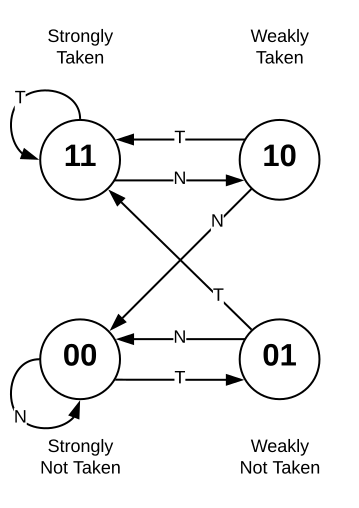
\includegraphics[scale =1] {figures/2bc-fsm}}
	\caption{ \small Two-bit counter state machine.}
	\label{fig:2bc-fsm}
\end{figure}

Although it's no longer strictly a ``counter", this change allows us to separate out the read and write requirements on the {\em prediction} and {\em hystersis} bits and place them in separate sequential memory tables. In hardware, the 2bc table can be implemented as follows:

\begin{quote}
The P-bit:
\begin{itemize}
\item {\bf read} - every cycle to make a prediction
\item {\bf write} - only when a misprediction occurred (the value of the h-bit).
\end{itemize}

The H-bit:

\begin{itemize}
\item {\bf read} - only when a misprediction occurred.
\item {\bf write} - when a branch is resolved (write the direction the branch took).
\end{itemize}
\end{quote}

By breaking the high-order p-bit and the low-order h-bit apart, we can place each in 1~read/1~write SRAM. A few more assumptions can help us do even better. Mispredictions are rare and branch resolutions are not necessarily occurring on every cycle. Also, writes can be delayed or even dropped altogether. Therefore, the {\em h-table} can be implemented using a single 1rw-ported SRAM by queueing writes up and draining them when a read is not being performed. Likewise, the {\em p-table} can be implemented in 1rw-ported SRAM by banking it -- buffer writes and drain when there is not a read conflict.


A final note: SRAMs are not happy with a ``tall and skinny'' aspect ratio that the 2bc tables require. However, the solution is simple -- tall and skinny can be trivially transformed into a rectangular memory structure.  The high-order bits of the index can correspond to the SRAM row and the low-order bits can be used to mux out the specific bits from within the row. 

\subsection{The GShare Predictor}

{\em Gshare} is a simple but very effective branch predictor. Predictions are made by hashing the instruction address and the global history (typically a simple XOR) and then indexing into a table of two-bit counters.  Figure \ref{fig:2bc-prediction} shows the logical architecture and Figure \ref{fig:gshare} shows the physical implementation and structure of the {\em gshare} predictor. Note that the prediction begins in the BP0 stage when the requesting address is sent to the predictor but that the prediction is made later in the BP2 stage once the instructions have returned from the instruction cache and the prediction state has been read out of the {\em gshare}'s p-table.


\begin{figure}[ht]
	\centering
	\centerline{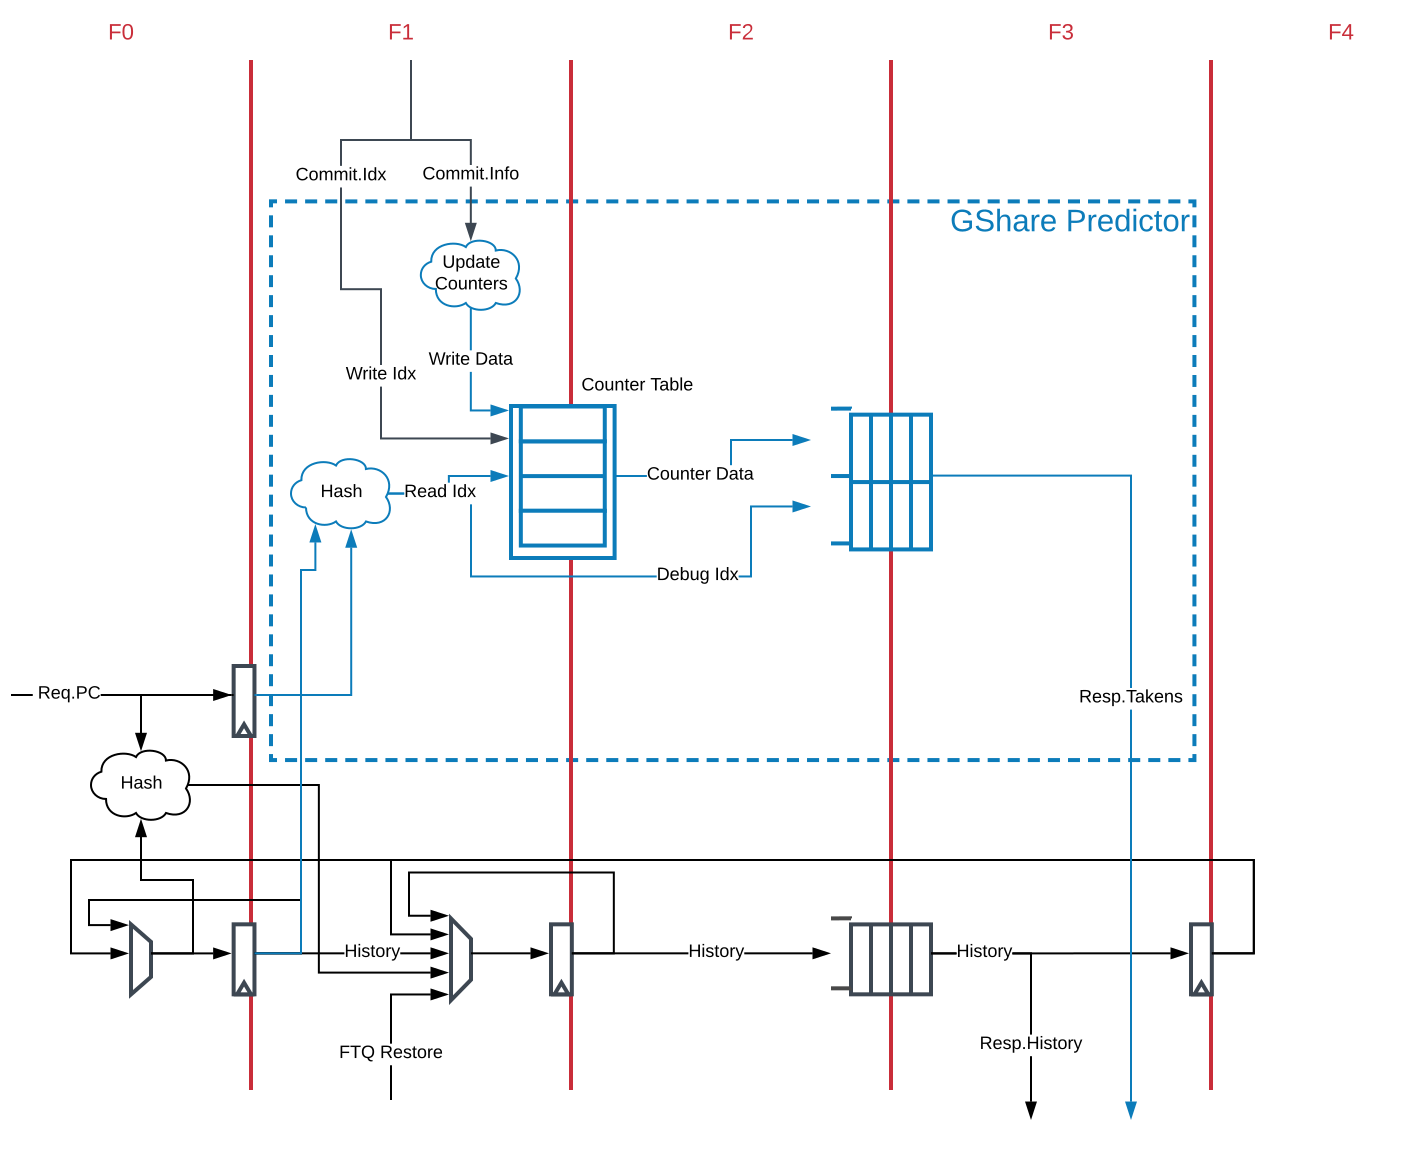
\includegraphics[scale =0.95] {figures/gshare}}
	\caption{ \small The GShare predictor pipeline.}
	\label{fig:gshare}
\end{figure}

\subsection{The TAGE Predictor}\label{sec:tage}

BOOM also implements the TAGE conditional branch predictor. TAGE is a highly-parameterizable, state-of-the-art global history predictor~\cite{seznec2006case, seznec2011new}.  The design is able to maintain a high degree of accuracy while scaling from very small predictor sizes to very large predictor sizes. It is fast to learn short histories while also able to learn very, very long histories (over a thousand branches of history).  


\begin{figure}[ht]
	\centering
	\centerline{\includegraphics[scale =0.80] {figures/tage}}
	\caption{ \small The TAGE predictor. The requesting address (PC) and the global history are fed into each table's index hash and tag hash. Each table provides its own prediction (or no prediction) and the table with the longest history wins.}
	\label{fig:tage}
\end{figure}


TAGE (TAgged GEometric) is implemented as a collection of predictor tables. Each table entry contains a {\em prediction counter}, a {\em usefulness counter}, and a {\em tag}. The {\em prediction counter} provides the prediction (and maintains some hysteresis as to how strongly biased the prediction is towards taken or not-taken). The {\em usefulness counter} tracks how useful the particular entry has been in the past for providing correct predictions.  The {\em tag} allows the table to only make a prediction if there is a tag match for the particular requesting instruction address and global history.

Each table has a different (and geometrically increasing) amount of history associated with it.  Each table's history is used to hash with the requesting instruction address to produce an index hash and a tag hash.  Each table will make its own prediction (or no prediction, if there is no tag match).  The table with the longest history making a prediction wins. 

On a misprediction, TAGE attempts to allocate a new entry. It will only overwrite an entry that is ``not useful'' ($ubits == 0$). 

\subsubsection{TAGE Global History and the Circular Shift Registers (CSRs)\protect\footnote{No relation to the Control/Status Registers.}}

Each TAGE table has associated with it its own global history (and each table has geometrically more history than the last table). As the histories become incredibly long (and thus too expensive to snapshot directly), TAGE uses the Very Long Global History Register (VLHR) as described in Section \ref{sec:vlhr}.  The histories contain many more bits of history that can be used to index a TAGE table; therefore, the history must be ``folded'' to fit. A table with 1024 entries uses 10 bits to index the table. Therefore, if the table uses 20 bits of global history, the top 10 bits of history are XOR'ed against the bottom 10 bits of history. 

Instead of attempting to dynamically fold a very long history register every cycle, the VLHR can be stored in a circular shift register (CSR).  The history is stored already folded and only the new history bit and the oldest history bit need to be provided to perform an update. Code \ref{code:tage-csr} shows an example of how a CSR works. 

\begin{center}
\begin{minipage}{0.90\textwidth}
\begin{lstlisting}[caption={The circular shift register. When a new branch outcome is added, the register is shifted (and wrapped around). The new outcome is added and the oldest bit in the history is ``evicted''.}]
Example:   
  A 12 bit value (0b_0111_1001_1111) folded onto a 5 bit CSR becomes 
  (0b_0_0010), which can be found by:                                       
                                                                             
                                                                             
               /-- history[12] (evict bit)                                   
               |                                                             
 c[4], c[3], c[2], c[1], c[0]                                                
  |                        ^                                                 
  |                        |                                                 
  \_______________________/ \---history[0] (newly taken bit)                 
                                                                             
                                                                             
(c[4] ^ h[ 0] generates the new c[0]).                                        
(c[1] ^ h[12] generates the new c[2]).       
\end{lstlisting}\label{code:tage-csr}
\end{minipage}
\end{center}                                 

Each table must maintain {\em three} CSRs.  The first CSR is used for computing the index hash and has a size $n=log(num\_table\_entries)$.  As a CSR contains the folded history, any periodic history pattern matching the length of the CSR will XOR to all zeroes (potentially quite common).  For this reason, there are two CSRs for computing the tag hash, one of width $n$ and the other of width $n-1$. 

For every prediction, all three CSRs (for every table) must be snapshotted and reset if a branch misprediction occurs. 
Another three {\em commit copies} of these CSRs must be maintained to handle pipeline flushes. 


\subsubsection{Usefulness counters (u-bits)}

The ``usefulness'' of an entry is stored in the {\em u-bit} counters.  Roughly speaking, if an entry provides a correct prediction, the u-bit counter is incremented. If an entry provides an incorrect prediction, the u-bit counter is decremented.  When a misprediction occurs, TAGE attempts to allocate a new entry.  To prevent overwriting a useful entry, it will only allocate an entry if the existing entry has a usefulness of zero.  However, if an entry allocation fails because all of the potential entries are useful, then all of the potential entries are decremented to potentially make room for an allocation in the future.

To prevent TAGE from filling up with only useful but rarely-used entries, TAGE must provide a scheme for ``degrading'' the u-bits over time.  A number of schemes are available.  One option is a timer that periodically degrades the u-bit counters.  Another option is to track the number of failed allocations (incrementing on a failed allocation and decremented on a successful allocation). Once the counter has saturated, all u-bits are degraded. 

\subsubsection{TAGE Snapshot State}

For every prediction, all three CSRs (for every table) must be snapshotted and reset if a branch misprediction occurs.  
TAGE must also remember the index of each table that was checked for a prediction (so the correct entry for each table can be updated later). 
Finally, TAGE must remember the tag computed for each table -- the tags will be needed later if a new entry is to be allocated.\footnote{There are ways to mitigate some of these costs, but this margin is too narrow to contain them.}
%\footnote{Although it is tempting to try and recompute the indices and tags to save on storage space, the problem with recomputing during {\em Commit} is that it would require having the {\em fetch PC} and the {\em fetch-time} values of the CSRs available to recreate the hashes.  As the CSRs are the most expensive part of the TAGE snapshots, they are deallocated after the branch is resolved in the {\em Execute} stage as they are only required for fixing a branch misprediction.}

\subsection{Other Predictors}

BOOM provides a number of other predictors that may provide useful.

\subsubsection{The Null Predictor}

The Null Predictor is used when no BPD predictor is desired. It will always predict ``not taken".

\subsubsection{The Random Predictor}

The Random Predictor uses an LFSR to randomize both ``was a prediction made?" and ``which direction each branch in the {\em fetch packet} should take?".  This is very useful for both torturing-testing BOOM and for providing a worse-case performance baseline for comparing branch predictors.

\section{Branch Prediction Configurations}

There are a number of parameters provided to govern the branch prediction in BOOM.

\subsection{GShare Configuration Options}

\subsubsection{Global History Length}

How long of a history should be tracked?  The length of the global history sets the size of the branch predictor. An $n$-bit history pairs with a $2^n$ entry two-bit counter table. 

\subsection{TAGE Configurations}

\subsubsection{Number of TAGE Tables}

How many TAGE tables should be used?

\subsubsection{TAGE Table Sizes}

What size should each TAGE table be?

\subsubsection{TAGE Table History Lengths}

How long should the global history be for each table? This should be a geometrically increasing value for each table.

\subsubsection{TAGE Table Tag Sizes}

What size should each tag be?

\subsubsection{TAGE Table U-bit Size}

How many bits should be used to describe the usefulness of an entry?


\chapter{The Decode Stage}

The decode stage takes instructions from the fetch buffer, decodes them, and allocates the necessary resources as required by each instruction.  The decode stage will stall as needed if not all resources are available.

%\section{The Decode Table}

%I think it would be neat to discuss how the decoder is essentially generated from a table, I don't know exactly how this works but it's honestly pretty neat and most companies are moving to table-based decoders (in excel normally I think), so this is a huge selling point of Chisel (not of BOOM directly, but it's related). Perhaps this section could be written by someone else

%\TODO{discuss the decode table}

%\section{Parameterization}

%The width of the Decode Stage is parameterizable.  However, the current limitation is the Fetch 
%\TODO{discuss parameterization, and the coupling of fetch width to decode width}.

%\TODO{discuss allocating branch tags and branch mask bits and other resources?}
\chapter{The Rename Stage}

The rename stage maps the {\em ISA} (or {\em logical}) register specifiers of each instruction to {\em physical} register specifiers. 

% discuss how this is an explicit renamed design
% discuss what renaming gets us (breaks all but true dependences)
% allows loop iterations to procceed in parallel, thanks to breaking the ``name" hazard

\section{The Purpose of Renaming}

{\em Renaming} is a technique to rename the ISA (or {\em logical}) register specifiers in an instruction by mapping them to a new space of {\em physical} registers.  The goal to {\em register renaming} is to break the output- (WAW) and anti-dependences (WAR) between instructions, leaving only the true dependences (RAW).  Said again, but in architectural terminology, register renaming eliminates write-after-write (WAW) and write-after-read (WAR) hazards, which are artifacts introduced by a) only having a limited number of ISA registers to use as specifiers and b) loops, which by their very nature will use the same register specifiers on every loop iteration. 

\section{The Explicit Renaming Design}

BOOM is an ``explicit renaming" or ``physical register file" out-of-order core design.  A physical register file, containing many more registers than the ISA dictates, holds both the committed architectural register state and speculative register state. The rename map tables contain the information needed to recover the committed state. As instructions are renamed, their register specifiers are explicitly updated to point to physical registers located in the physical register file.\footnote{The MIPS R10k\cite{mipsr10k}, Alpha 21264\cite{alpha21264}, Intel Sandy Bridge, and ARM Cortex A15 cores are all example of explicit renaming out-of-order cores.}


\begin{figure}[htb]
	\centering
	\centerline{\includegraphics[scale =0.8] {figures/prf-and-arf}}
	\caption{ \small A PRF design (left) and a data-in-ROB design (right).}
	\label{fig:prf_design}
\end{figure}
%\TODO{redo drawing without the +1 to reduce confusion}


This is in contrast to an ``implicit renaming" or ``data-in-ROB" out-of-order core design.  The Architectural Register File (ARF) only holds the committed register state, while the ROB holds the speculative write-back data.  On commit, the ROB transfers the speculative data to the ARF. \footnote{The Pentium 4 and the ARM Cortex A57 are examples of {\em implicit renaming} designs.}




\begin{figure}[htb]
	\centering
	\centerline{\includegraphics[scale =0.6] {figures/rename-pipeline}}
	\caption{ \small The Rename Stage. Logical register specifiers read the map table to get their physical specifier. For superscalar rename, any changes to the map tables must be bypassed to dependent instructions. The physical source specifiers can then read the Busy Table. The {\em Stale} specifier is used to track which physical register will be freed when the instruction later commits. P0 in the Physical Register File is always 0.}
	\label{fig:rename-pipeline}
\end{figure}
%TODO{remove lrd, and change to ldst?}


\section{The Rename Map Table}

The Rename Map Table holds the speculative mappings from ISA registers to physical registers.  

Each branch gets its own copy of the rename map table.\footnote{An alternate design for wider pipelines may prefer to only make up to one snapshot per cycle, but this comes with additional complexity to deduce the precise mappings for any given instruction within the fetch packet.}  On a branch mispredict, the map table can be reset instantly from the mispredicting branch's copy of the map table. 

As the RV64G ISA uses fixed locations of the register specifiers (and no implicit register specifiers), the map table can be read before the instruction is decoded!  

\subsection{Resets on Exceptions and Flushes}


An additional, optional ``Committed Map Table" holds the rename map for the committed architectural state.  If enabled, this allows single-cycle reset of the pipeline during flushes and exceptions (the current map table is reset to the committed map table). Otherwise, pipeline flushes require multiple cycles to ``unwind" the ROB to write back in the rename state at the commit point, one ROB row per cycle.


\section{The Busy Table}

The Busy Table tracks the readiness status of each physical register. If all physical operands are ready, the instruction will be ready to be issued. 

\section{The Free List}

The free-list tracks the physical registers that are currently un-used and is used to allocate new physical registers to instructions passing through the {\em Rename} stage.  

The Free List is implemented as a bit-vector.  A priority decoder can then be used to find the first free register. BOOM uses a cascading priority decoder to allocate multiple registers per cycle.\footnote{A two-wide rename stage could use two priority decoders starting from opposite ends.}

On every branch (or jalr), the rename map tables are snapshotted to allow single-cycle recovery on a branch misprediction. Likewise, the Free List also sets aside a new ``Allocation List", initialized to zero.  As new physical registers are allocated, the Allocation List for each branch is updated to track all of the physical registers that have been allocated after the branch. If a misspeculation occurs, its Allocation List is added back to the Free List by {\em OR'ing} the branch's Allocation List with the Free List.\footnote{Conceptually, branches are often described as ``snapshotting" the Free List (along with an {\em OR'ing} with the current Free List at the time of the misprediction). However, snapshotting fails to account for physical registers that were allocated when the snapshot occurs, then become freed, then becomes re-allocated before the branch mispredict is detected.  In this scenario, the physical register gets leaked, as neither the snapshot nor the current Free List know that it had been freed.  Eventually, the processor slows as it struggles to maintain enough inflight physical registers, until finally the machine comes to a halt. If this sounds autobiographical because the author may have trusted computer architecture lectures, well...}

\section{Stale Destination Specifiers}

For instructions that will write a register, the map table is read to get the {\em stale physical destination specifier} (``stale pdst").  Once the instruction commits, the {\em stale pdst} is returned to the free list, as no future instructions will read it.

%\section{Handling Branch Mispredictions}
%
%Every instruction in the pipeline has a ``branch mask", which is a bit-vector describing each live branch that it is currently being speculated under. Each branch is allocated a ``branch tag", and a corresponding branch mask bit such that every following instruction will have that corresponding bit set in its own branch mask.  Once a branch is resolved, the corresponding branch mask bit is cleared in every instruction's branch-mask. If the branch is misspeculated, then all instructions with the corresponding branch mask bit is killed. 




\chapter{The Reorder Buffer (ROB) and the Dispatch Stage}\label{chapter:rob}


The ROB tracks the state of all inflight instructions in the pipeline. The role of the ROB is to provide the illusion to the programmer that his program executes in-order. 
After instructions are decoded and renamed, they are then dispatched to the ROB and the issue window and marked as {\em busy}. 
As instructions finish execution, they inform the ROB and are marked {\em not busy}. 
Once the ``head" of the ROB is no longer busy, the instruction is {\em committed}, and it's architectural state now visible. If an exception occurs and the excepting instruction is at the head of the ROB, the pipeline is flushed and no architectural changes that occurred after the excepting instruction are made visible. The ROB then redirects the PC to the appropriate exception handler. 

\section{The ROB Organization}

The ROB is, conceptually, a circular buffer that tracks all inflight instructions in-order. The oldest instruction is pointed to by the {\em commit head}, and the newest instruction will be added at the {\em rob tail}. 

To facilitate superscalar {\em Dispatch} and {\em Commit}, the ROB is implemented as a circular buffer with $W$ banks (where $W$ is the {\em dispatch} and {\em commit} width of the machine\footnote{This design sets up the {\em Dispatch} and {\em Commit} widths of BOOM to be the same. However, that is not necessarily a fundamental constraint, and it would be possible to orthogonalize the {\em Dispatch} and {\em Commit} widths, just with more added control complexity.}). This organization is shown in Figure \ref{fig:rob}. 

%\subsection{Dispatch}

At {\em dispatch}, up to $W$ instructions are written from the {\em fetch packet} into an ROB row, where each instruction is written to a different bank across the row.  As the instructions within a {\em fetch packet} are all consecutive (and aligned) in memory, this allows a single PC to be associated with the entire {\em fetch packet} (and the instruction's position within the {\em fetch packet} provides the low-order bits to its own PC).  While this means that branching code will leave bubbles in the ROB, it makes adding more instructions to the ROB very cheap as the expensive costs are amortized across each ROB row.

%An entire {\em fetch packet} is decoded, renamed, and then dispatched together.\footnote{This is not strictly true, as it is possible, say due to a lack of resources, for some of the instructions to be dispatched before the full {\em fetch packet} can be dispatched.} 
%This constraint couples the {\em Fetch Width} to the {\em Decode}, {\em Rename}, and {\em Dispatch} widths. 


\begin{figure}[htb]
	\centering
	\centerline{\includegraphics[scale =1] {figures/rob}}
	\caption{ \small The Reorder Buffer for a two-wide BOOM with three-issue. Dispatched uops ({\em dis\_uops}) are written at the bottom of the ROB ({\em rob\_tail}), while committed uops ({\em com\_uops}) are committed from the top, at {\em rob\_head}, and update the rename state. Uops that finish executing ({\em wb\_uops}) clear their {\em busy} bit. {\bf Note:} the dispatched uops are written into the same ROB row together, and are located consecutively in memory allowing a single PC to represent the entire row. }
	\label{fig:rob}
\end{figure}

\section{ROB State}

Each ROB entry contains relatively little state:

\begin{itemize}
\item is entry valid?
\item is entry busy?
\item is entry an exception?
\item branch mask (which branches is this entry still speculated under? 
\item rename state (what is the logical destination and the stale physical destination?)
\item floating-point status updates
\item other miscellaneous data (e.g., helpful for statistic tracking)
\end{itemize}

The PC and the branch prediction information is stored on a per-row basis (see Sec \ref{sec:pcstorage}).  The Exception State only tracks the oldest known excepting instruction (see Sec \ref{sec:rob_xcpt}). 

\subsection{Exception State}\label{sec:rob_xcpt}

The ROB tracks the oldest excepting instruction. If this instruction reaches the head of the ROB, then an exception is thrown. 

Each ROB entry is marked with a single-bit to signify whether or not the instruction has encountered exceptional behavior, but the additional exception state (e.g., the bad virtual address and the exception cause) is only tracked for the oldest known excepting instruction.  This saves considerable state by not storing this on a per entry basis. 

\subsection{PC Storage}\label{sec:pcstorage}

The ROB must know the PC of every inflight instruction.  This information is used in the following situations:

\begin{itemize}
\item Any instruction could cause an exception, in which the ``exception pc" (epc) must be known.
\item Branch and jump instructions need to know their own PC for for target calculation.
\item Jump-register instructions must know both their own PC {\bf and the PC of the following instruction} in the program to verify if the front-end predicted the correct JR target.
\end{itemize}

This information is incredibly expensive to store. Instead of passing PCs down the pipeline, branch and jump instructions access the ROB's ``PC File" during the {\em Register-read} stage for use in the Branch Unit. Two optimizations are used:


\begin{itemize}
\item only a single PC is stored per ROB row.\footnote{Because instructions within an ROB row are consecutive in the program, the instruction's ROB bank implicitly provides the lower PC bits.}
\item the PC File is stored in two banks, allowing a single read-port to read two consecutive entries simultaneously (for use with JR instructions).
\end{itemize}

\section{The Commit Stage}

When the instruction at the {\em commit head} is no longer busy (and it is not excepting), it may be {\em committed}, i.e., its changes to the architectural state of the machine are made visible. For superscalar commit, the entire ROB row is analyzed for {\em not busy} instructions (and thus, up to the entire ROB row may be committed in a single cycle). The ROB will greedily commit as many instructions as it can per row to release resource as soon as possible. However, the ROB does not (currently) look across multiple rows to find commit-able instructions. 

Only once a store has been committed may it be sent to memory. For superscalar committing of stores, the LSU is told ``how many stores" may be marked as committed. The LSU will then drain the committed stores to memory as it sees fit. 

When an instruction (that writes to a register) commits, it then frees the {\em stale physical destination register}. The {\em stale pdst} is then free to be re-allocated to a new instruction. 


\section{Exceptions and Flushes}

Exceptions are handled when the instruction at the {\em commit head} is excepting. The pipeline is then flushed and the ROB emptied. The rename map tables must be reset to represent the true, non-speculative {\em committed} state. The front-end is then directed to the appropriate PC.  If it is an architectural exception, the excepting instruction's PC (referred to as the {\em exception vector}) is sent to the Control/Status Register file.  If it is a micro-architectural exception (e.g., a load/store ordering misspeculation) the failing instruction is refetched and execution can begin anew. 

\subsection{Parameterization - Rollback versus Single-cycle Reset}

The behavior of resetting the map tables is parameterizable.  The first option is to rollback the ROB one row per cycle to unwind the rename state (this is the behavior of the MIPS R10k\cite{mipsr10k}).  For each instruction, the {\em stale physical destination} register is written back into the map table for its {\em logical destination} specifier. 

A faster single-cycle reset is available.  This is accomplished by using another rename snapshot that tracks the {\em committed} state of the rename tables. This {\em committed map table} is updated as instructions commit.\footnote{The tradeoff here is between longer latencies on exceptions versus an increase in area and wiring.}

\subsection{Causes}

The RV64G ISA provides relatively few exception sources:

\begin{quote}
\begin{description}
\item[Load/Store Unit] - page faults
\item[Branch Unit] - misaligned fetches
\item[Decode Stage] - all other exceptions and interrupts can be handled before the instruction is dispatched to the ROB
\end{description}
\end{quote}

Note that memory ordering speculation errors also originate from the Load/Store Unit, and are treated as exceptions in the BOOM pipeline (actually they only cause a pipeline ``retry"). 

\include{sections/issue}
\chapter{The Register File and Bypass Network}

BOOM is a unified, physical register file (PRF) design. The register file holds both the committed and speculative state. The register file also holds both integer and floating point register values. The map tables track which physical register corresponds to which ISA register. 

BOOM uses the Berkeley hardfloat floating point units which use an internal 65-bit operand format (\url{https://github.com/ucb-bar/berkeley-hardfloat}).  Therefore, all physical registers are 65-bits.



\begin{figure}[htb]
	\centering
	\centerline{\includegraphics[scale =0.8] {figures/1w-rrd-bypass-pipeline}}
	\caption{ \small An example single-issue pipeline. The register file needs 3 read ports to satisfy FMA operations and 2 write ports to satisfy the variable latency operations without interfering with the fixed latency ALU and FP write-backs. To make scheduling of the write port trivial, the ALU's pipeline is lengthened to match the FPU latency.  The ALU is able to bypass from any of these stages to dependent instructions in the {\em Register Read} stage. }
	\label{fig:1w-rrd-bypass-pipeline}
\end{figure}


\section{Register Read}

The register file statically provisions all of the register read ports required to satisfy all issued instructions. For example, if {\em issue port \#0} corresponds to an integer ALU and {\em issue port \#1} corresponds to a FPU, then the first two register read ports will statically serve the ALU and the next three register read ports will service the FPU for five total read ports. 

\subsection{Dynamic Read Port Scheduling}

Future designs can improve area-efficiency by provisioning fewer register read ports and using dynamically scheduling to arbitrate for them. This is particularly helpful as most instructions need only one operand.  However, it does add extra complexity to the design, which is often manifested as extra pipeline stages to arbitrate and detect structural hazards.  It also requires the ability to kill issued micro-ops and re-issue them from the issue window on a later cycle. 

\section{Bypass Network}

ALU operations can be issued back-to-back by having the write-back values forwarded through the bypass network. Bypassing occurs at the end of the {\em Register Read} stage. 




\chapter{The Execute Pipeline}\label{chapter:execute}

%when wakeup occurs?

The Execution Pipeline covers the execution and write-back of micro-ops.  Although the micro-ops will travel down the pipeline one after the other (in the order they have been issued), the micro-ops themselves are likely to have been issued to the Execution Pipeline out-of-order. Figure \ref{fig:execute-pipeline} shows an example Execution Pipeline for a dual-issue BOOM. 

\begin{figure}[htbp]
	\centering
	\centerline{\includegraphics[scale =0.75] {figures/execution-pipeline-2w}}
	\caption{ \small An example pipeline for a dual-issue BOOM. The first issue port schedules micro-ops onto Execute Unit \#0, which can accept ALU operations, FPU operations, and integer multiply instructions.  The second issue port schedules ALU operations, integer divide instructions (unpipelined), and load/store operations.  The ALU operations can bypass to dependent instructions.  Note that the ALU in EU\#0 is padded with pipeline registers to match latencies with the FPU and iMul units to make scheduling for the write-port trivial. Each Execution Unit has a single issue-port dedicated to it but contains within it a number of lower-level Functional Units.}
	\label{fig:execute-pipeline}
\end{figure}



\section{Execution Units}


\begin{figure}[htbp]
	\centering
	\centerline{\includegraphics[scale =0.8] {figures/execution-unit}}
	\caption{ \small An example Execution Unit. This particular example shows an integer ALU (that can bypass results to dependent instructions) and an unpipelined divider that becomes {\em busy} during operation. Both functional units share a single write-port.  The Execution Unit accepts both {\em kill} signals and {\em branch resolution} signals and passes them to the internal functional units as required.}
	\label{fig:execute-unit}
\end{figure}


An Execution Unit is a module that a single issue port will schedule micro-ops onto and contains some mix of functional units.  Phrased in another way, each issue port from the Issue Window talks to one and only one Execution Unit. An Execution Unit may contain just a single simple integer ALU, or it could contain a full complement of floating point units, a integer ALU, and an integer multiply unit.  

The purpose of the Execution Unit is to provide a flexible abstraction which gives a lot of control over what kind of Execution Units the architect can add to their pipeline

\subsection{Scheduling Readiness}

An Execution Unit provides a bit-vector of the functional units it has available to the issue scheduler. The issue scheduler will only schedule micro-ops that the Execution Unit supports.  For functional units that may not always be ready (e.g., an un-pipelined divider), the appropriate bit in the bit-vector will be disabled (See Fig \ref{fig:execute-unit}).



\section{Functional Units}

Functional units are the muscle of the CPU, computing the necessary operations as required by the instructions.  Functional units typically require a knowledgable domain expert to implement them correctly and efficiently.  


\begin{figure}[htbp]
	\centering
	\centerline{\includegraphics[scale =0.9] {figures/abstract-functional-unit}}
	\caption{ \small The abstract Pipelined Functional Unit class. An expert-written, low-level functional unit is instantiated within the Functional Unit. The request and response ports are abstracted and bypass and branch speculation support is provided. Micro-ops are individually killed by gating off their response as they exit the low-level functional unit.}
	\label{fig:abstract-functional-unit}
\end{figure}


For this reason, BOOM uses an abstract Functional Unit class to ``wrap" expert-written, low-level functional units from the Rocket repository (see Section \ref{sec:rocket}).  However, the expert-written functional units created for the Rocket in-order processor make assumptions about in-order issue and commit points (namely, that once an instruction has been dispatched to them it will never need to be killed). These assumptions break down for BOOM.

However, instead of re-writing or forking the functional units, BOOM provides an abstract Functional Unit class (see Fig \ref{fig:abstract-functional-unit}) that ``wraps" the lower-level functional units with the parameterized auto-generated support code needed to make them work within BOOM. The request and response ports are abstracted, allowing Functional Units to provide a unified, interchangeable interface.  

\subsection{Pipelined Functional Units}

A pipelined functional unit can accept a new micro-op every cycle. Each micro-op will take a known, fixed latency. 

Speculation support is provided by auto-generating a pipeline that passes down the micro-op meta-data and {\em branch mask} in parallel with the micro-op within the expert-written functional unit. If a micro-op is misspeculated, it's response is de-asserted as it exits the functional unit. 

An example pipelined functional unit is shown in Fig \ref{fig:abstract-functional-unit}.

\subsection{Un-pipelined Functional Units}

Un-pipelined functional units (e.g., a divider) take an variable (and unknown) number of cycles to complete a single operation. Once occupied, they de-assert their ready signal and no additional micro-ops may be scheduled to them. 

Speculation support is provided by tracking the {\em branch mask} of the micro-op in the functional unit. 

The only requirement of the expert-written un-pipelined functional unit is to provide a {\em kill} signal to quickly remove misspeculated micro-ops.\footnote{This constraint could be relaxed by waiting for the un-pipelined unit to finish before de-asserting its busy signal and suppressing the {\em valid} output signal.}

\begin{figure}[htbp]
	\centering
	\centerline{\includegraphics[scale =0.75] {figures/functional-unit-hierarchy}}
	\caption{ \small The dashed ovals are the low-level functional units written by experts, the squares are concrete classes that instantiate the low-level functional units, and the octagons are abstract classes that provide generic speculation support and interfacing with the BOOM pipeline. The floating point divide and squart-root unit doesn't cleanly fit either the Pipelined nor Unpipelined abstract class, and so directly inherits from the FunctionalUnit super class.}
	\label{fig:functional-unit-hierarchy}
\end{figure}




\section{Branch Unit \& Branch Speculation}

The Branch Unit handles the resolution of all branch and jump instructions.  

All micro-ops that are ``inflight" in the pipeline (have an allocated ROB entry) are given a {\em branch mask}, where each bit in the {\em branch mask} corresponds to an un-executed, inflight branch that the micro-op is speculated under. Each branch in {\em Decode} is allocated a {\em branch tag}, and all following micro-ops will have the corresponding bit in the {\em branch mask} set (until the branch is resolved by the Branch Unit). 

If the branches (or jumps) have been correctly speculated by the front-end, then the Branch Unit's only action is to broadcast the corresponding branch tag to {\em all} inflight micro-ops that the branch has been resolved correctly.  Each micro-op can then clear the corresponding bit in its {\em branch mask}, and that branch tag can then be allocated to a new branch in the {\em Decode} stage. 

If a branch (or jump) is misspeculated, the Branch Unit must redirect the PC to the correct target, kill the front-end and fetch buffer, and broadcast the misspeculated {\em branch tag} so that all dependent, inflight micro-ops may be killed.  The PC redirect signal goes out immediately, to decrease the misprediction penalty.  However, the {\em kill} signal is delayed a cycle for critical path reasons. 

The front-end must pass down the pipeline the appropriate branch speculation meta-data, so that the correct direction can be reconciled with the prediction.  Jump Register instructions are evaluated by comparing the correct target with the PC of the next instruction in the ROB (if not available, then a misprediction is assumed).  Jumps are evaluated and handled in the front-end (as their direction and target are both known once the instruction can be decoded). 

% TODO{do jumps need to be in the pipeline at all? what about in-correct branch target exceptions?}

BOOM (currently) only supports having one Branch Unit. %Relaxing this constraint would add more ports to the ROB PC File. 

\section{Load/Store Unit}.

The Load/Store Unit (LSU) handles the execution of load, store, atomic, and fence operations. 

BOOM (currently) only supports having one LSU (and thus can only send one load or store per cycle to memory).\footnote{Relaxing this constraint could be achieved by allowing multiple LSUs to talk to their own bank(s) of the data-cache, but the added complexity comes in allocating entries in the LSU before knowing the address, and thus which bank, a particular memory operation pertains to.}

See Chapter \ref{sec:lsu} for more details on the LSU.

\section{Floating Point Units}

\begin{figure}[htbp]
	\centering
	\centerline{\includegraphics[scale =0.9] {figures/functional-unit-fpu}}
	\caption{ \small The class hierarchy of the FPU is shown. The expert-written code is contained within the {\tt hardfloat} and {\tt rocket} repositories. The ``FPU" class instantiates the Rocket components, which itself is further wrapped by the abstract Functional Unit classes (which provides the out-of-order speculation support).}
	\label{fig:functional-unit-fpu}
\end{figure}

The low-level floating point units used by BOOM come from the Rocket processor (\url{https://github.com/ucb-bar/rocket}) and hardfloat (\url{https://github.com/ucb-bar/berkeley-hardfloat}) repositories.  Figure \ref{fig:functional-unit-fpu} shows the class hierarchy of the FPU. 

To make the scheduling of the write-port trivial, all of the pipelined FP units are padded to have the same latency.\footnote{Rocket instead handles write-port scheduling by killing and refetching the offending instruction (and all instructions behind it) if there is a write-port hazard detected. This would be far more heavy-handed to do in BOOM.}

\section{Floating Point Divide and Square-root Unit}

BOOM fully supports floating point divide and square-root operations using a single ``{\tt {FDiv/Sqrt}}" (or \fdiv\ for short).  BOOM accomplishes this by instantiating a double-precision {\tt {divSqrtRecF64}} unit from the {\tt hardfloat} repository.  The {\tt {divSqrtRecF64}} unit comes with the following features/constraints:

\begin{itemize}
\item expects 65-bit recoded double-precision inputs
\item provides a 65-bit recoded double-precision output
\item can execute a divide operation and a square-root operation simultaneously
\item operations are unpipelined and take an unknown, variable latency
\item provides an {\em unstable} FIFO interface
\end{itemize}

Single-precision operations have their operands upscaled to double-precision (and then the output downscaled).\footnote{It is cheaper to perform the SP-DP conversions than it is to instantiate a single-precision fdivSqrt unit.}

Although the \fdiv\ unit is unpipelined, it does not fit cleanly into the Pipelined/Unpipelined abstraction used by the other functional units (Fig \ref{fig:functional-unit-hierarchy}).  This is because the {\tt {divSqrtRecF64}} unit provides an unstable FIFO interface: although the \fdiv\ unit may provide a {\em ready} signal on Cycle $i$, there is no guarantee that it will continue to be {\em ready} on Cycle $i+1$, even if no operations are enqueued. This proves to be a challenge, as the issue window may attempt to issue an \fdiv\ instruction but cannot be certain the \fdiv\ unit will  accept it once it reaches the \fdiv\ unit on a later cycle.  

The solution is to add extra buffering within the \fdiv\ unit to hold instructions until they can be released directly into the {\tt {divSqrtRecF64}} unit. If the buffering of the \fdiv\ unit fills up, back pressure can be safely applied to the issue window.\footnote{It is this ability to hold multiple inflight instructions within the \fdiv\ unit simultaneously that breaks the ``only one instruction at a time" assumption required by the UnpipelinedFunctionalUnit abstract class.}

%\footnote{The \fdiv\ unit cannot inherent from the PipelinedFunctionalUnit class, as it is not pipelined and don't make use of any of the auto-generated pipeline speculation support infrastructure. However, it also cannot inherent from the UnpipelinedFunctionalUnit class, because it's auto-generated infrastructure assumes that only one micro-op will be present in the functional unit at any given point in time. The \fdiv\ unit, with its unstable interface (which demands extra buffering) and ability to support divide and square-root operations simultaneously, requires hand-writing its own speculation support code and thus inherits directly from the high-level FunctionalUnit abstract class (as it still maintains the same high-level interfaces).}

\section{Parameterization}

BOOM provides flexibility in specifying the issue width and the mix of functional units in the execution pipeline. Code \ref{code:exe_units} shows how to instantiate an execution pipeline in BOOM.
  
\begin{center}
\begin{minipage}{0.66\textwidth}
\begin{lstlisting}[caption=Instantiating the Execution Pipeline (in {\tt dpath.scala}). Adding execution units is as simple as instantiating another ExecutionUnit module and adding it to the {\tt exe\_units} ArrayBuffer.]
val exe_units = ArrayBuffer[ExecutionUnit]()

if (ISSUE_WIDTH == 2)
{
   exe_units += Module(new ALUExeUnit(is_branch_unit = true
                                       , has_mul     = true
                                       ))
   exe_units += Module(new ALUMemExeUnit(has_div     = true
                                       ))
}
else if (ISSUE_WIDTH == 3)
{
   exe_units += Module(new ALUExeUnit(is_branch_unit = true
                                       , has_mul     = true
                                       ))
   exe_units += Module(new ALUExeUnit(has_div = true))
   exe_units += Module(new MemExeUnit())
}
\end{lstlisting}\label{code:exe_units}
\end{minipage}
\end{center}

Additional parameterization, regarding things like the latency of the FP units can be found within the Configuration settings ({\tt configs.scala}).



\section{Control/Status Register Instructions}

A set of Control/Status Register (CSR) instructions allow the atomic read and write of the Control/Status Registers.  These architectural registers are separate from the integer and floating registers, and include the cycle count, retired instruction count, status, exception PC, and exception vector registers (and many more!).  Each CSR has its own required privilege levels to read and write to it and some have their own side-effects upon reading (or writing).  

BOOM (currently) does not rename {\em any} of the CSRs, and in addition to the potential side-effects caused by reading or writing a CSR, {\bf BOOM will only execute a CSR instruction non-speculatively.}\footnote{There is a lot of room to play with regarding the CSRs. For example, it is probably a good idea to rename the {\tt {sscratch}} register (dedicated for use by the supervisor) as it may see a lot of use in some kernel code and it causes no side-effects.}  This is accomplished by marking the CSR instruction as a ``unique" (or ``serializing") instruction - the ROB must be empty before it may proceed to the Issue Window (and no instruction may follow it until it has finished execution and been committed by the ROB).  It is then issued by the Issue Window, reads the appropriate operands from the Physical Register File, and is then sent to the CSRFile.\footnote{The CSRFile is a Rocket component.}  The CSR instruction executes in the CSRFile and then writes back data as required to the Physical Register File. The CSRFile may also emit a PC redirect and/or an exception as part of executing a CSR instruction (e.g., a {\tt syscall}). 

\include{sections/lsu}
\include{sections/memory}
\chapter{Micro-architectural Event Tracking}

Version 1.9.1 of the RISC-V Privileged Architecture adds support for Hardware Performance Monitor (HPM) counters.\footnote{Future efforts may add some counters into a memory-mapped access region. This will open up the ability to track events that, for example, may not be tied to any particular core (like last-level cache misses).}  The HPM support allows a nearly infinite number of micro-architectural events to be multiplexed onto up to 29 physical counters.  The privilege access levels can also be set on a per-counter basis.

\begin{table}[htp]
\caption{Uarch Events}
\begin{center}
\begin{tabular}{|c|c|}
\hline
Number & Event \\
\hline
\hline
1 & Committed Branches  \\
\hline
2 & Committed Branch Mispredictions\\
\hline
... & and many more (see core.scala) \\
\hline
\end{tabular}
\end{center}
\label{table:uarchcounters}
\end{table}%

The available events can be modified in {\tt core.scala} as desired.\footnote{Note: {\tt io.events(0)} will get mapped to being {\tt Event \#1} (etc.) from the point of view of the RISC-V software.}  It is then up to machine-level software to set the privilege access level and the {\em event selectors} for each counter as desired.

\begin{center}
\begin{minipage}{0.66\textwidth}
\begin{lstlisting}[caption=Setting the privilege level and event selectors for the HPM counters.]
static void mstatus_init()
{
   // Enable user/supervisor use of perf counters
   write_csr(mucounteren, -1);
   write_csr(mscounteren, -1);

   // set events 1 and 2 to counters 3 and 4.
   write_csr(mhpmevent3, 1);
   write_csr(mhpmevent4, 2);
\end{lstlisting}\label{ref:code_hpm_init}
\end{minipage}
\end{center}


\section{Reading HPM Counters in Software}

The Code Example \ref{ref:code_uarch} demonstrates how to read the value of any CSR register from software.
  
  
\begin{center}
\begin{minipage}{0.66\textwidth}
\begin{lstlisting}[caption=Reading a CSR register.]
#define read_csr_safe(reg) ({ register long __tmp asm("a0"); \   
  asm volatile ("csrr %0, " #reg : "=r"(__tmp)); \               
  __tmp; })             
  
  long csr_cycle  = read_csr_safe(cycle);
  long csr_instr  = read_csr_safe(instret);
  long csr_hpmc3  = read_csr_safe(hpmcounter3);
  ...
  long csr_hpmc31 = read_csr_safe(hpmcounter31);
  
\end{lstlisting}\label{ref:code_uarch}
\end{minipage}
\end{center}



\chapter{Verification}

This chapter covers the current recommended techniques for verifying BOOM.  Although not provided as part of the BOOM or rocket-chip repositories, it is also recommended that BOOM be tested on ``hello-world + riscv-pk" and the RISC-V port of Linux to properly stress the processor.

\section{RISC-V Tests}

A basic set of functional tests and micro-benchmarks can be found at (\url{https://github.com/riscv/riscv-tests}).  These are invoked by the ``make run" targets in the emulator, fsim, and vsim directories. 

\section{RISC-V Torture Tester}

Berkeley's {\tt riscv-torture} tool is used to stress the BOOM pipeline, find bugs, and provide small code snippets that can be used to debug the processor. Torture can be found at (\url{https://github.com/ucb-bar/riscv-torture}).

\

\begin{quote}
{\bf Quick-start}

\texttt{\#} compile the BOOM C++ emulator

\texttt{\$} \verb=cd rocket-chip/emulator; make run CONFIG==\verb=BOOMCPPConfig=

\

\texttt{\#} check out and run the {\tt riscv-torture} repository

\texttt{\$} \verb=cd ../          # top-level rocket-chip directory=

\texttt{\$} \verb=git clone https://github.com/ucb-bar/riscv-torture.git=

\texttt{\$} \verb=cd riscv-torture=

\texttt{\$} \verb=git submodule update --init=

\texttt{\$} \verb=vim Makefile    # change RTL_CONFIG==\verb=BOOMCPPConfig=

\texttt{\$} \verb=make igentest   # test that torture works, gen a single test=

\texttt{\$} \verb=make cnight     # run C++ emulator overnight=
\end{quote}



\chapter{Debugging}
\include{sections/visualization}
\chapter{Physical Realization}\label{chapter:physical}

This chapter provides information useful for physically realizing the BOOM processor.  Although BOOM VLSI work is very preliminary, it has been synthesized at 1~GHz on a high-end mobile 28~nm process. Unfortunately, while VLSI flows are difficult to share or make portable (and encumbered with proprietary libraries and tools), an enterprising individual may want to visit the \url{https://github.com/ucb-bar/plsi} portable ``Palmer's VLSI Scripts'' repository which describes one way to push BOOM through a VLSI flow.

\section{Register Retiming}
 
Many VLSI tools require the designer to manually specify which modules need to
be analyzed for retiming. 
                 
In BOOM, the floating point units and the pipelined integer multiply unit are
described combinationally and then padded to the requested latency with
registers.
In order to meet the desired clock frequency,  {\bf the floating point units and the
pipelined integer multiply unit must be register-retimed}.
 
\begin{center}
\begin{minipage}{0.90\textwidth}
\begin{lstlisting}[caption=Pipelined integer multiply unit requires register retiming to be realized properly.]
val mul_result = lhs.toSInt * rhs.toSInt
                                                                               
val mul_output_mux = MuxCase(                                                  
   UInt(0, 64), Array(                                                         
      FN(DW_64, FN_MUL)    -> mul_result(63,0),                                
      FN(DW_64, FN_MULH)   -> mul_result(127,64),                              
      FN(DW_64, FN_MULHU)  -> mul_result(127,64),                              
      FN(DW_64, FN_MULHSU) -> mul_result(127,64),                              
      FN(DW_32, FN_MUL)    -> Cat(Fill(32, mul_result(31)), mul_result(31,0)), 
      FN(DW_32, FN_MULH)   -> Cat(Fill(32, mul_result(63)), mul_result(63,32)),
      FN(DW_32, FN_MULHU)  -> Cat(Fill(32, mul_result(63)), mul_result(63,32)),
      FN(DW_32, FN_MULHSU) -> Cat(Fill(32, mul_result(63)), mul_result(63,32)) 
))                                                                             
                                                                               
io.out := ShiftRegister(mul_output_mux, imul_stages, io.valid)
\end{lstlisting}\label{code:imul}
\end{minipage}
\end{center}

\section{Pipelining Configuration Options}

Although BOOM does not provide high-level configurable-latency pipeline stages, BOOM does provide a few configuration options to help the implementor trade off CPI performance for cycle-time. 

\subsubsection{EnableFetchBufferFlowThrough}

The front-end fetches instructions and places them into a {\em fetch buffer}.  The back-end pulls instructions out of the fetch buffer and then decodes, renames, and dispatches the instructions into the {\em issue window}. This fetch buffer can be optionally set to be a {\em flow-through} queue -- instructions enqueued into the buffer can be immediately dequeued on the other side on the same clock cycle.  Turning this option {\bf off} forces all instructions to spend at least one cycle in the queue but decreases the critical path between instruction fetch and dispatch.

\subsubsection{EnableBrResolutionRegister}

The branch unit resolves branches, detects mispredictions, fans out the branch kill signal to {\em all} inflight micro-ops, redirects the PC select stage to begin fetching down the correct path, and sends snapshot information to the branch predictor to reset its state properly so it can begin predicting down the correct path.  Turning this option {\bf on} delays the branch resolution by a cycle.  In particular, this adds a cycle to the branch misprediction penalty (which is hopefully a rare event).

\subsubsection{Functional Unit Latencies}

The latencies of the pipelined floating point units and the pipelined integer multiplier unit can be modified.  Currently, all floating point unit latencies are set to the latency of the longest floating point unit (i.e., the DFMA unit).  This can be changed by setting the {\em dfmaLatency} in the {\em FPUConfig} class. Likewise, the integer multiplier is also set to the {\em dfmaLatency}.\footnote{The reason for this is that the imul unit is most likely sharing a write port with the DFMA unit and so must be padded out to the same length. However, this isn't fundamental and there's no reason an imul unit not sharing a write port with the FPUs should be constrained to their latencies.}


\appendix
\include{sections/futurework}
\chapter{Parameterization}\label{chapter:parameterization}

\section{Rocket Parameters}
\section{BOOM Parameters}
\section{Uncore Parameters}

\chapter{Frequently Asked Questions}

To be filled in as questions are asked!

\include{sections/terminology}


\begin{figure}[ht]
	\centering
	\centerline{\includegraphics[scale =.9, angle=90] {figures/simple_boom_pipeline}}
	\caption{ \small A more detailed diagram of BOOM, for a single-issue RV32IM design.}
	\label{fig:boom-detailed}
\end{figure}






%\begin{scriptsize}
\bibliographystyle{abbrv}
\bibliography{bibliography}
%\end{scriptsize}


\end{document}
